\chapter{Módem BLU por Método de Desfase}
\label{sec:desarrollo_blu}

En este capítulo se analiza la modulación de Banda Lateral Única (BLU o SSB)
mediante el método de desfase , y su posterior demodulación sincrónica. El
esquema circuital simulado en Multisim se presenta en la fig.
\ref{crkt.blu:circuito}.

\begin{figure}[!ht]
    \centering
    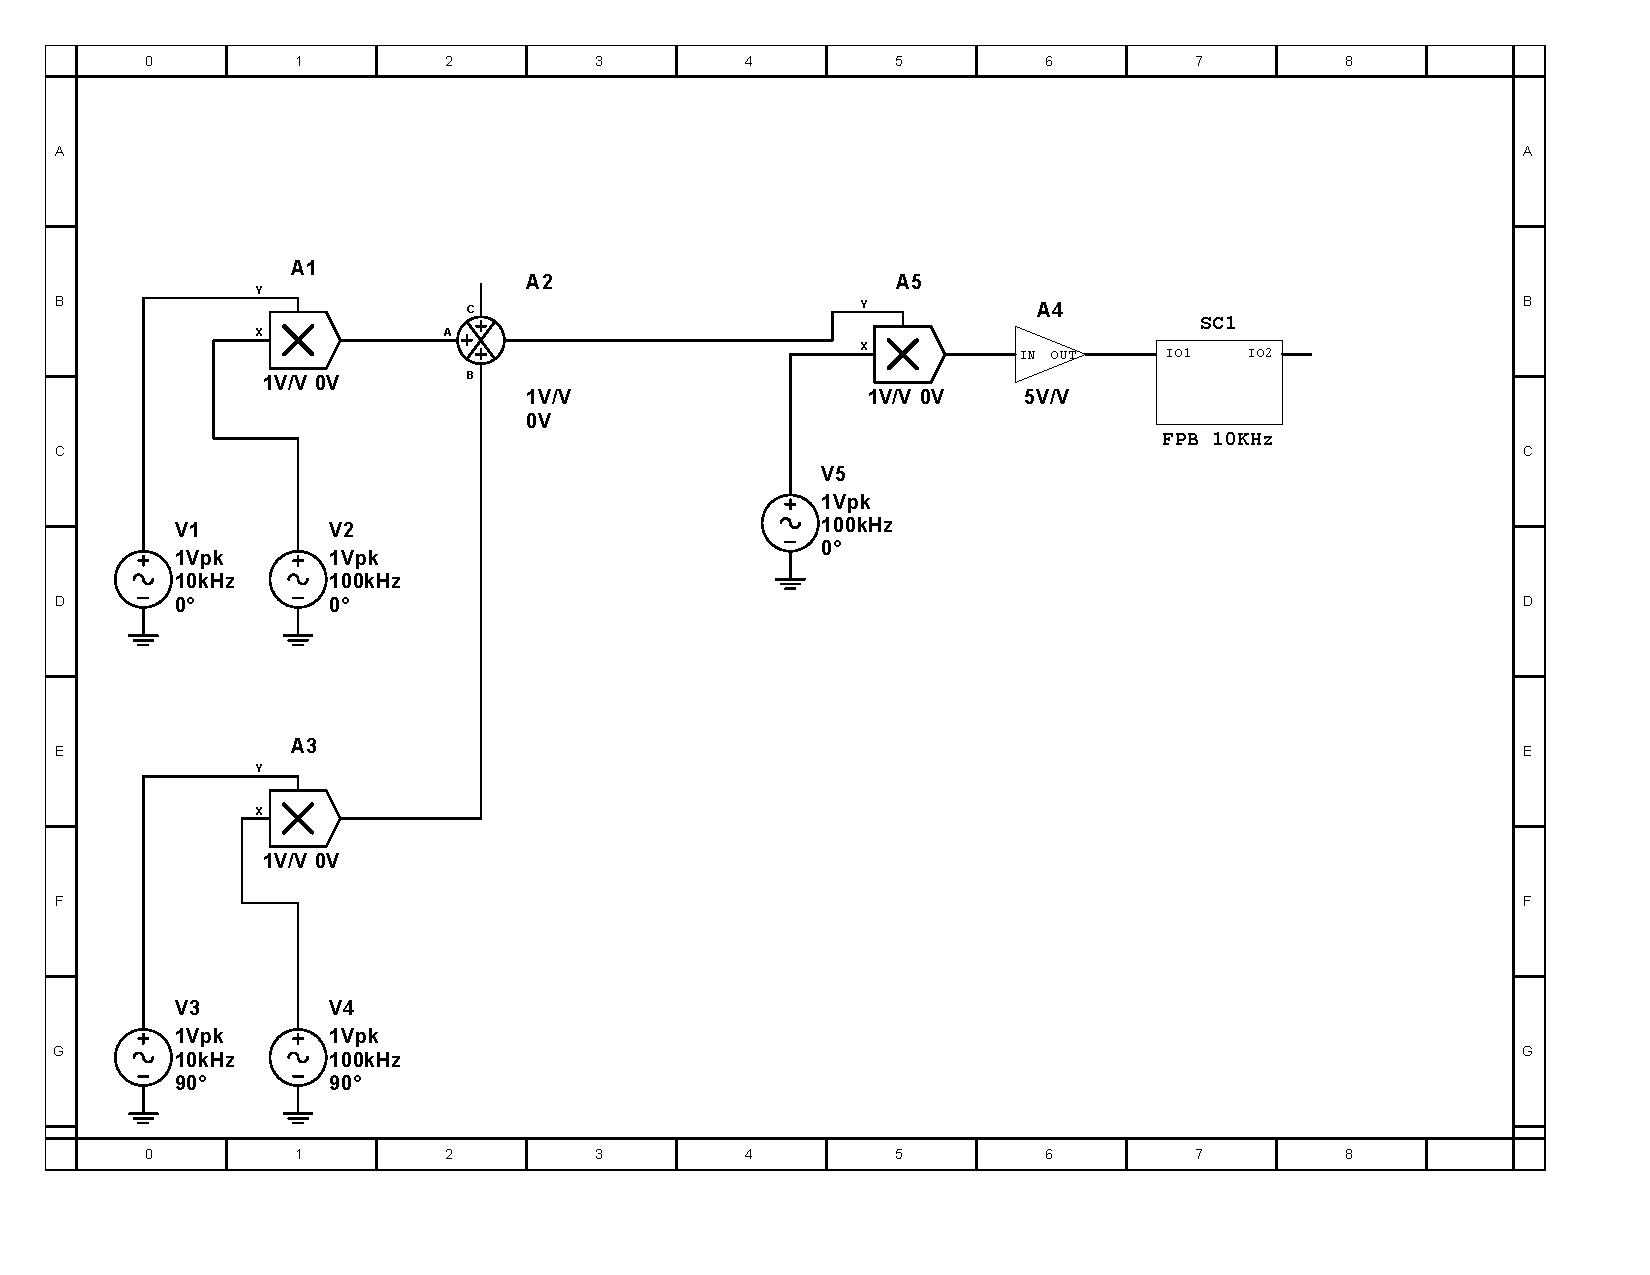
\includegraphics[width=0.95\textwidth]{images/tp1b_circuit.pdf}
    \caption{Circuito del módem BLU implementado en Multisim.}
    \label{crkt.blu:circuito}
\end{figure}

\section{Modulación BLU por el Método de Desfase}

Este método de modulación utiliza dos ramas en cuadratura para generar una señal BLU sin necesidad de filtros de
banda ultra-selectivos. Sus componentes principales son:
\begin{itemize}
    \item \textbf{Rama Directa (En Fase):} Multiplica la señal modulante $m(t) = A_m \cos(\omega_m t)$ con la
          portadora $c(t) = A_c \cos(\omega_c t)$. Esto produce el producto en fase en el \textbf{Punto de Medición C}:
          \begin{equation}
              v_d(t) = A_m A_c \cos(\omega_m t) \cos(\omega_c t) = \frac{A_m A_c}{2} [\cos(\omega_c - \omega_m)t + \cos(\omega_c + \omega_m)t]
          \end{equation}
    \item \textbf{Rama en Cuadratura (Desfasada $90^\circ$):} Multiplica la señal modulante desfasada
          $-90^\circ$, dada por $\hat{m}(t) = A_m \sin(\omega_m t)$, con la portadora desfasada $-90^\circ$, dada por
          $\hat{c}(t) = A_c \sin(\omega_c t)$. Esto produce el producto en cuadratura en el \textbf{Punto de Medición D}:
          \begin{equation}
              v_q(t) = A_m A_c \sin(\omega_m t) \sin(\omega_c t) = \frac{A_m A_c}{2} [\cos(\omega_c - \omega_m)t - \cos(\omega_c + \omega_m)t]
          \end{equation}
\end{itemize}

Sumando o restando ambas señales se obtiene la señal BLU deseada en el \textbf{Punto de Medición E}:
\begin{equation}
    s_{\text{BLU}}(t) = v_d(t) \mp v_q(t)
\end{equation}

\begin{itemize}
    \item \textbf{Banda Lateral Superior (BLS o USB):} Se obtiene mediante la resta:
          \begin{equation}
              s_{\text{USB}}(t) = v_d(t) - v_q(t) = A_m A_c \cos(\omega_c + \omega_m)t
          \end{equation}
          El espectro consta de una única componente en $f_c + f_m = 110\kHz$.
    \item \textbf{Banda Lateral Inferior (BLI o LSB):} Se obtiene mediante la suma:
          \begin{equation}
              s_{\text{LSB}}(t) = v_d(t) + v_q(t) = A_m A_c \cos(\omega_c - \omega_m)t
          \end{equation}
          El espectro consta de una única componente en $f_c - f_m = 90\kHz$.
\end{itemize}

\subsection{Puntos de Medición del Módem}
En la simulación se configuran los siguientes puntos de prueba distribuidos a lo largo del modulador y demodulador:
\begin{itemize}
    \item \textbf{Punto A:} Señal modulante en banda base ($1\V$ - $10\kHz$).
    \item \textbf{Punto B:} Señal portadora ($1\V$ - $100\kHz$).
    \item \textbf{Punto C:} Salida del multiplicador de la rama directa (AM con portadora suprimida).
    \item \textbf{Punto D:} Salida del multiplicador de la rama en cuadratura (producto de la portadora y la modulante desfasadas $90^\circ$).
    \item \textbf{Punto E:} Salida del sumador/restador (señal BLU resultante).
    \item \textbf{Punto F:} Salida del mezclador del receptor (demodulación sincrónica previa al filtro).
    \item \textbf{Punto G:} Salida del filtro pasa-bajos del receptor (señal demodulada recuperada).
\end{itemize}

\begin{figure}[!ht]
    \centering
    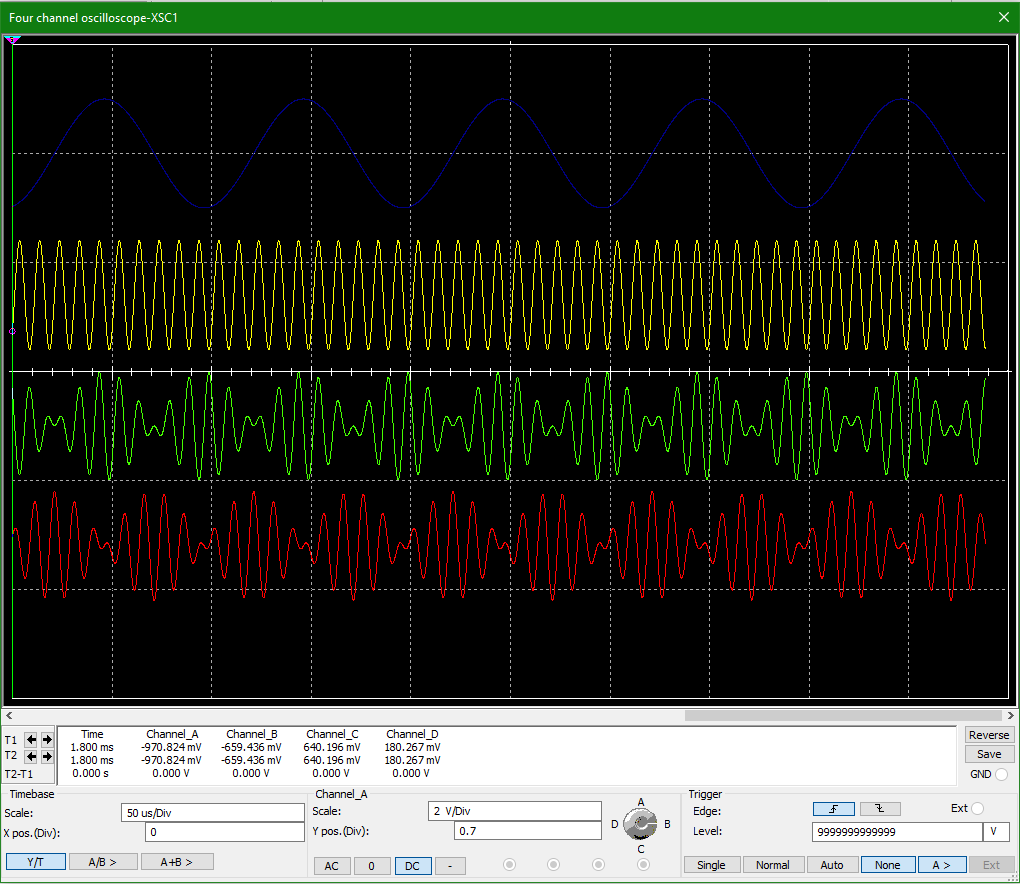
\includegraphics[width=0.85\textwidth]{images/Mediciones_ABCD_tp1_b.png}
    \caption{Medición en el dominio del tiempo de los Puntos A (modulante), B (portadora), C (salida rama directa) y D (salida rama en cuadratura) en un único gráfico.}
    \label{fig.blu:mediciones_abcd}
\end{figure}

\begin{figure}[!ht]
    \centering
    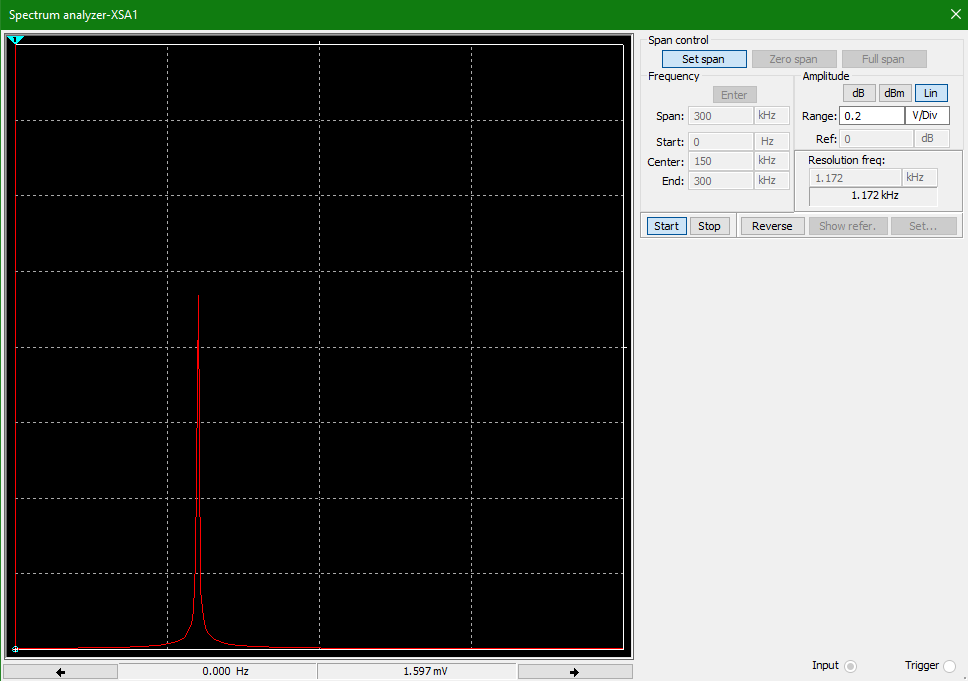
\includegraphics[width=0.75\textwidth]{images/Medicion_E_tp1_b.png}
    \caption{Espectro de la señal BLU resultante a la salida del modulador (Punto E).}
    \label{fig.blu:puntoE}
\end{figure}

\section{Análisis de los Efectos de Modificación de Amplitud (Punto A)}
Si se modifica la amplitud de la señal modulante en banda base $A_m$ en el Punto A, la amplitud de la señal BLU
resultante cambia de manera directamente proporcional.
Dado que el modulador es lineal en amplitud, no se generan frecuencias espurias ni distorsión armónica si el
desfasaje de $90^\circ$ se mantiene ideal. El espectro de la señal BLU mostrará simplemente un aumento o disminución
del nivel de la banda lateral seleccionada, sin alterar la supresión de la banda lateral no deseada.

\section{Análisis del Efecto de Desfasamiento Imperfecto (Error de Fase)}
En un modulador real, es difícil mantener un desfasaje exacto de $90^\circ$ en todas las frecuencias. Se analiza el
caso en el que existe un error de fase, simulando un desfasamiento de $80^\circ$ (error de fase $\theta_e = 10^\circ$)
en lugar de los $90^\circ$ teóricos.

\subsection{Derivación Matemática de la Relación Banda Lateral Deseada a No Deseada}
Supongamos que la señal en cuadratura tiene un error de fase $\theta_e$, de forma que la diferencia de fase total
entre las ramas de modulación es $\phi = 90^\circ - \theta_e$. Las señales de salida de los multiplicadores son:
\begin{gather*}
    v_d(t) = \frac{1}{2} [\cos(\omega_c t - \omega_m t) + \cos(\omega_c t + \omega_m t)] \\
    v_q(t) = \cos(\omega_m t - (90^\circ - \theta_e))\cos(\omega_c t - 90^\circ)
\end{gather*}

Usando identidades trigonométricas se puede demostrar que al combinar las ramas para obtener, por ejemplo, la
señal de banda lateral superior (USB) mediante resta, la amplitud de la banda deseada ($A_{\text{deseada}}$)
y la de la banda no deseada ($A_{\text{no\_deseada}}$) son:
\begin{gather}
    A_{\text{deseada}} = \cos\left(\frac{\theta_e}{2}\right) \\
    A_{\text{no\_deseada}} = \sin\left(\frac{\theta_e}{2}\right)
\end{gather}

La relación de rechazo o supresión de la banda lateral no deseada en decibelios (dB) se define como:
\begin{equation}
    R_{\text{dB}} = 20 \log_{10} \left( \frac{A_{\text{no\_deseada}}}{A_{\text{deseada}}} \right) = 20 \log_{10} \left( \tan\left(\frac{\theta_e}{2}\right) \right)
    \label{eq.blu:supresion_fase}
\end{equation}

Para el caso solicitado con un desfase de $80^\circ$, el error es $\theta_e = 10^\circ$. Evaluando eq. \ref{eq.blu:supresion_fase}:
\begin{equation}
    R_{\text{dB}} = 20 \log_{10} \left( \tan(5^\circ) \right) \approx 20 \log_{10} (0.08749) \approx -21.16\text{ dB}
\end{equation}

Este resultado indica que un error de fase de solo $10^\circ$ degrada severamente la supresión de la banda lateral
no deseada, la cual pasa de ser idealmente infinita a ser de solo $-21.16\text{ dB}$ por debajo de la deseada.

\section{Demodulación de BLU}
La demodulación de la señal BLU es sincrónica. Requiere multiplicar la señal BLU recibida por una portadora local
sincronizada en frecuencia y fase con la portadora original ($100\kHz$, fase $0^\circ$).
Al multiplicar la señal de USB, se obtiene en el \textbf{Punto de Medición F}:
\begin{equation}
    v_{\text{dem}}(t) = s_{\text{USB}}(t) \cos(2\pi f_c t) = A_m A_c \cos(2\pi (f_c + f_m) t) \cos(2\pi f_c t)
\end{equation}
\begin{equation}
    v_{\text{dem}}(t) = \frac{A_m A_c}{2} [\cos(2\pi f_m t) + \cos(2\pi (2f_c + f_m) t)]
\end{equation}

\begin{figure}[!ht]
    \centering
    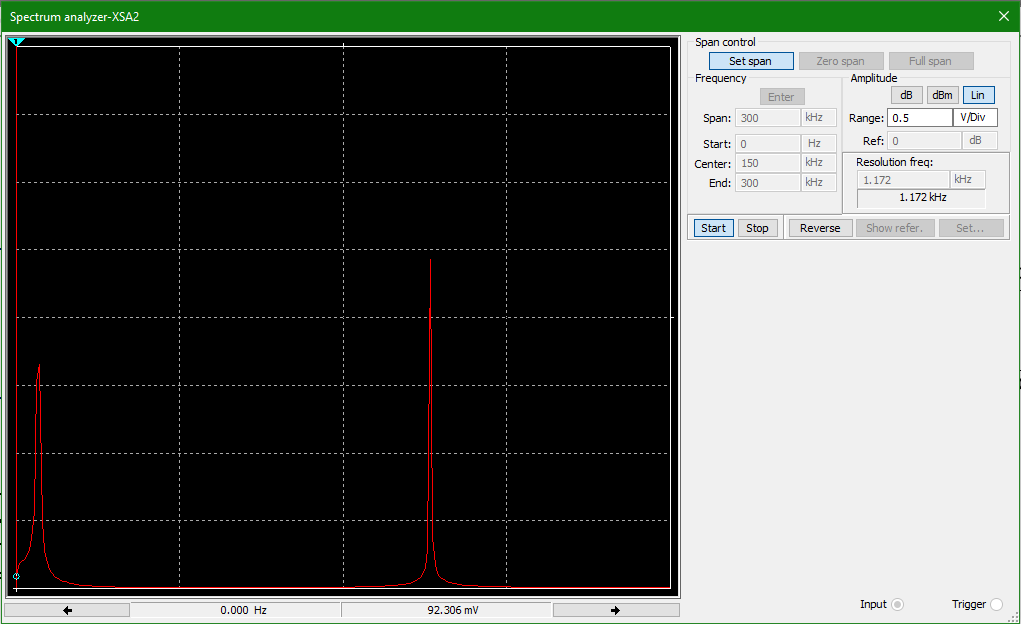
\includegraphics[width=0.75\textwidth]{images/Medicion_F_tp1_b.png}
    \caption{Espectro de la señal a la salida de la demodulación sincrónica previa al filtrado (Punto F).}
    \label{fig.blu:puntoF}
\end{figure}

Un filtro pasa-bajos posterior con frecuencia de corte de $10\kHz$ elimina la componente de alta frecuencia
($2f_c + f_m = 210\kHz$), permitiendo recuperar la modulante original en el \textbf{Punto de Medición G}:
\begin{equation}
    v_{\text{out}}(t) = \frac{A_m A_c}{2} \cos(2\pi f_m t)
\end{equation}

\begin{figure}[!ht]
    \centering
    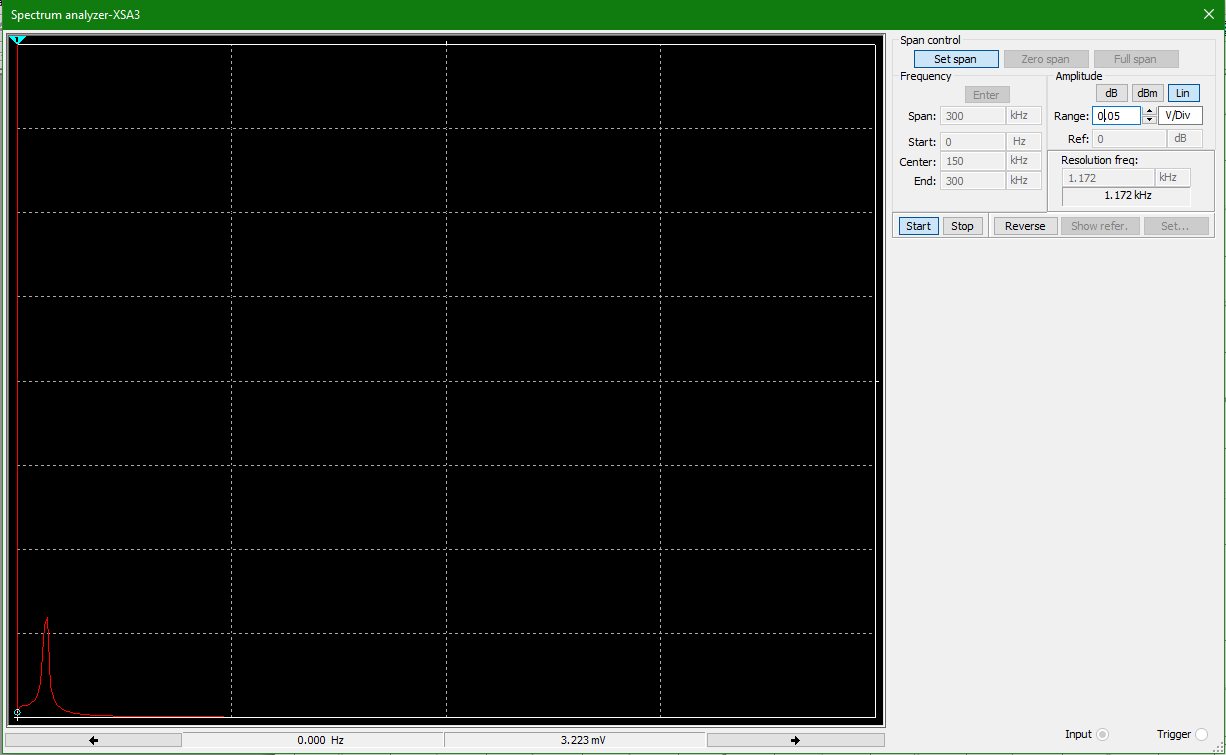
\includegraphics[width=0.75\textwidth]{images/Medicion_G_tp1_b.png}
    \caption{Señal recuperada tras el demodulador BLU (Punto G) en el dominio de la frecuencia.}
    \label{fig.blu:demodulada}
\end{figure}
